%% Exemplo de utilizacao do estilo de formatacao normas-utf-tex (http://normas-utf-tex.sourceforge.net)
%% Autores: Hugo Vieira Neto (hvieir@utfpr.edu.br)
%%          Diogo Rosa Kuiaski (diogo.kuiaski@gmail.com)
%% Colaboradores:
%%          Cézar M. Vargas Benitez <cesarvargasb@gmail.com>
%%          Marcos Talau <talau@users.sourceforge.net>


\documentclass[openright]{abnt-UTFPR-PPGCA-proj} %openright = o capitulo comeca sempre em paginas impares
%\documentclass[openright]{normas-utf-tex} %openright = o capitulo comeca sempre em paginas impares
%\documentclass[oneside]{normas-utf-tex} %oneside = para dissertacoes com numero de paginas menor que 100 (apenas frente da folha) 


\usepackage[alf,abnt-emphasize=bf,bibjustif,recuo=0cm, abnt-etal-cite=2, abnt-etal-list=99]{abntcite} %configuracao correta das referencias bibliograficas.

\usepackage[brazil]{babel} % pacote portugues brasileiro
\usepackage[utf8]{inputenc} % pacote para acentuacao direta
\usepackage{amsmath,amsfonts,amssymb} % pacote matematico
\usepackage{graphicx} % pacote grafico
%\usepackage{times} % fonte times
\usepackage{arial} % fonte arial
\usepackage{url}

%Podem utilizar GEOMETRY{...} para realizar pequenos ajustes das margens. Onde, left=esquerda, right=direita, top=superior, bottom=inferior. P.ex.:
%\geometry{left=3.0cm,right=1.5cm,top=4cm,bottom=1cm} 

% ---------- Preambulo ----------
\instituicao{Universidade Tecnol\'ogica Federal do Paran\'a} % nome da instituicao
\area{Computa\c{c}\~ao Aplicada} % [Engenharia Biom\'edica] ou [Inform\'atica Industrial] ou [Telem\'atica]
\programa{Programa de P\'os-gradua\c{c}\~ao em Computa\c{c}\~ao Aplicada} % nome do programa
\departamento{Departamento Acad\^emico de Inform\'atica} % departamento

\documento{Projeto de Disserta\c{c}\~ao de Mestrado} % {Semin\'ario de Acompanhamento I} ou {Semin\'ario de Acompanhamento II}
\nivel{Mestrado} % [Mestrado] ou [Doutorado]
\titulacao{Mestre} % [Mestre] ou [Doutor]

\titulo{T\'itulo em Portugu\^es} % titulo do trabalho em portugues
\title{Title in English} % titulo do trabalho em ingles

\author{Nome do Autor}
\autor{Nome do Autor}
\cita{SOBRENOME, Nome} % sobrenome (maiusculas), nome do autor do trabalho

\palavraschave{Palavra-chave 1, Palavra-chave 2, ...} % palavras-chave do trabalho
\keywords{Keyword 1, Keyword 2, ...} % palavras-chave do trabalho em ingles

\comentario{\UTFPRdocumentodata\ apresentada ao \UTFPRprogramadata\ da \ABNTinstituicaodata\ como requisito parcial para obten\c{c}\~ao do grau de ``\UTFPRtitulacaodata\ em Ci\^encias'' -- \'Area de Concentra\c{c}\~ao: \UTFPRareadata.}

\orientador{Nome do Orientador} % nome do orientador do trabalho
%\orientador[Orientadora:]{Nome da Orientadora} % <- no caso de orientadora, usar esta sintaxe
%\coorientador{Nome do Co-orientador} % nome do co-orientador do trabalho, caso exista
%\coorientador[Co-orientadora:]{Nome da Co-orientadora} % <- no caso de co-orientadora, usar esta sintaxe
%\coorientador[Co-orientadores:]{Nome do Co-orientador} % no caso de 2 co-orientadores, usar esta sintaxe
%\coorientadorb{Nome do Co-orientador 2}	% este comando inclui o nome do 2o co-orientador

\local{Curitiba} % cidade
\data{\the\year} % ano automatico


%---------- Inicio do Documento ----------
\begin{document}
\sloppy

\capa % geracao automatica da capa
%\folhaderosto % geracao automatica da folha de rosto
%\termodeaprovacao % <- ainda a ser implementado corretamente

% dedicatória (opcional)
%\begin{dedicatoria}
%Texto da dedicat\'oria.
%\end{dedicatoria}

% agradecimentos (opcional)
%\begin{agradecimentos}
%Texto dos agradecimentos.
%\end{agradecimentos}

% epigrafe (opcional)
%\begin{epigrafe}
%Texto da ep\'igrafe.
%\end{epigrafe}

%resumo
\begin{resumo}
Texto do resumo (m\'aximo de 500 palavras).

% Trecho extraído do modelo http://www2.dainf.ct.utfpr.edu.br/ppgca/estrutura-academica/regulamentacao/avaliacao/copy_of_ModeloProjetoeSeminarios.doc/view
Elemento obrigatório, formado por uma sequência de frases objetivas e concisas. Podem-se ressaltar os objetivos, metodologia aplicada, resultados e conclusões. Deve ser redigido em parágrafo único, com no máximo 500 palavras. Deve ser seguido de palavras chaves.
%-------------------------------------------------------------------------------
\end{resumo}

%abstract
\begin{abstract}
Abstract text (maximum of 500 words).
\end{abstract}

% listas (opcionais, mas recomenda-se a partir de 5 elementos)
\listadefiguras % geracao automatica da lista de figuras
\listadetabelas % geracao automatica da lista de tabelas
\listadesiglas % geracao automatica da lista de siglas
\listadesimbolos % geracao automatica da lista de simbolos

% sumario
\sumario % geracao automatica do sumario


%---------- Inicio do Texto ----------
% recomenda-se a escrita de cada capitulo em um arquivo texto separado (exemplo: intro.tex, fund.tex, exper.tex, concl.tex, etc.) e a posterior inclusao dos mesmos no mestre do documento utilizando o comando \input{}, da seguinte forma:
%---------- Primeiro Capitulo ----------
\chapter{Introdu\c{c}\~ao}
\label{chap:intro}

O presente documento \'e um exemplo de uso do estilo de formata\c{c}\~ao \LaTeX\ elaborado para atender \`as Normas para Elabora\c{c}\~ao de Trabalhos Acad\^emicos da UTFPR. O estilo de formata\c{c}\~ao {\ttfamily normas-utf-tex.cls} tem por base o pacote \textsc{abn}\TeX~-- cuja leitura da documenta\c{c}\~ao \cite{abnTeX2009} \'e fortemente sugerida~-- e o estilo de formata\c{c}\~ao \LaTeX\ da UFPR.

Para melhor entendimento do uso do estilo de formata\c{c}\~ao {\ttfamily normas-utf-tex.cls}, aconselha-se que o potencial usu\'ario analise os comandos existentes no arquivo \TeX\ ({\ttfamily modelo\_*.tex}) e os resultados obtidos no arquivo PDF ({\ttfamily modelo\_*.pdf}) depois do processamento pelo software \LaTeX\ + \textsc{Bib}\TeX~\cite{LaTeX2009,BibTeX2009}. Recomenda-se a consulta ao material de refer\^encia do software para a sua correta utiliza\c{c}\~ao~\cite{Lamport1986,Buerger1989,Kopka2003,Mittelbach2004}.

% Trecho extraído do modelo http://www2.dainf.ct.utfpr.edu.br/ppgca/estrutura-academica/regulamentacao/avaliacao/copy_of_ModeloProjetoeSeminarios.doc/view
A redação do plano de pesquisa ou proposta deve refletir o poder de síntese do seu autor. Utilize as formatações de página, espaçamento e fonte aqui apresentados (Fonte Arial 12, espaçamento entre linhas 1,5, folha tamanho A4, margens padrão do Word). 
Deve haver especial atenção com o índice, pois o mesmo é gerado de maneira automática, não devendo ser apagado. Depois de introduzir todos os seus textos sob os itens apropriados, coloque o cursor do mouse sobre a área onde está o índice, clique com o botão direito do mouse, selecione a opção “Atualizar campo” e depois “Atualizar apenas o número das páginas”. Pronto, o Índice indicará as páginas automaticamente. Não é preciso editá-lo. 
O texto de introdução deve conter três tipos de informações: apresentação do problema, estado da arte e justificativa do projeto. Uma vez que nem sempre é clara a linha divisória entre estes três tópicos, optou-se pela construção de uma seção única de introdução que deverá conter todas as informações acima mencionadas, permitindo ao autor elaborar um texto com fluência lógica e sem redundância de informações.
A apresentação ou formulação do problema deve deixar, de forma bem clara, qual será o objeto de estudo do projeto. As razões para a escolha do tema deverão ser justificadas e, para isso, você deverá discorrer sobre a importância do estudo, quais as possíveis repercussões, quais hipóteses a serem verificadas, etc. 
O estado da arte serve para embasar tanto a formulação do problema como sua justificativa. É preciso situar historicamente a evolução do tema, quais as abordagens já investigadas, qual o estágio atual do conhecimento sobre o assunto ou quais as tendências que se apresentam.
A justificativa do projeto deve indicar por que o projeto deve ser feito. Descreva os fatores de motivação que o levaram a abordar e trabalhar no assunto.
As maneiras mais comuns de citações são a indireta e a direta. Na citação indireta, o texto é criado com base na obra de autor consultado, no qual se reproduz o conteúdo e as idéias do documento original. Exemplo, utilizando Sobrenome do Autor (data), quando o nome do autor faz parte do texto: Segundo Souza (1999), a importância do tema [...]. Exemplo, utilizando (SOBRENOME DO AUTOR, ano) quando é citada a síntese de uma informação: A Revolução Industrial modificou definitivamente o cenário urbano (SOUZA, 2001). Na citação direta há a reprodução exata do texto citado entre aspas, como, por exemplo: A justificativa deste comportamento “é resultado da integração entre parasita e hospedeiro, após a conclusão da fase de migração” (SOUZA, 1987). No capítulo Referências, ao final deste documento, há diversos exemplos para apresentação da fonte de uma referência. Dúvidas e maiores detalhes, vide norma ABNT vigente para citações e referências.
Importante: O formato recomendado para as citações e referências é o ABNT. Consulte o orientador para verificar a necessidade de utilização de um formato de citações e de referências diferente, como a norma Vancouver.
Importante: Todos os trabalhos que envolvem seres humanos (inclusive entrevistas) e animais deverão obter aprovação do Comitê de Ética em Pesquisa (CEP) e devem apresentar uma cópia do Termo de Consentimento Informado (TCI), que deve ser assinado pelos participantes da pesquisa. Os requisitos do comitê de ética local estão à disposição no CEP, disponível em http://www.utfpr.edu.br/estrutura-universitaria/pro-reitorias/proppg/comite-de-etica-em-pesquisa-1 . O TCI é o documento em que são informadas aos participantes da pesquisa, em linguagem simples e acessível, todas as implicações possíveis (passadas, presentes ou futuras) da pesquisa para esta pessoa. Ao assinar este termo a pessoa estará autorizando sua inclusão na pesquisa. De modo semelhante, as pesquisas que envolverem animais devem respeitar integralmente os preceitos éticos para experimentação animal. 
O projeto de pesquisa deve estar submetido ao Comitê de Ética em Pesquisa o mais cedo possível, para não inviabilizar os prazos da conclusão do mestrado.
Importante: O Direito Autoral deve ser respeitado. A Constituição da República Federativa do Brasil, em seu Artigo 5, Parágrafo XXVII, indica (BRASIL, 1988): "aos autores pertence o direito exclusivo de utilização, publicação ou reprodução de suas obras, transmissível aos herdeiros pelo tempo que a lei fixar.". A Lei de Direitos Autorais (BRASIL, 1998) afirma:
Art 1º. Esta Lei regula os direitos autorais, entendendo-se sob esta denominação os direitos do autor e os que lhe são conexos.
Art. 7º. São obras intelectuais protegidas as criações de espírito, expressas por qualquer meio ou fixadas em qualquer suporte, tangível ou intangível, conhecido ou que se invente no futuro, como:
I - os textos de obras literárias, artísticas ou científicas;
Art. 22. Pertencem ao autor os direitos morais e patrimoniais sobre a obra que criou.
Art 29. Depende da autorização prévia e expressa do autor a utilização da obra, por quaisquer modalidades, tais como: 
I- a reprodução parcial ou integral;
II- a edição; 
Art. 41. Os direitos patrimoniais do autor perduram por setenta anos contados de 1º de janeiro do ano subsequente ao de seu falecimento, obedecida a ordem sucessória da lei civil.
Art. 46 - Não constitui ofensa aos direitos autorais: 
III - a citação em livros, jornais, revistas ou qualquer outro meio de comunicação, de passagens de qualquer obra, para fins de estudo, crítica ou polêmica, na medida justificada para o fim a atingir, indicando-se o nome do autor e a origem da obra;
A Lei n. 6895, de 17 de dezembro de 1980, que modifica o Código Penal, indica em seu artigo 184 (BRASIL, 1980):
Art. 184 - Violar direito autoral: 
Pena - detenção de 3 meses a 1 ano, ou multa.
§ 1º - Se a violação consistir na reprodução, por qualquer meio, com intuito de lucro, de obra intelectual, no todo ou em parte, sem autorização expressa do autor ou de quem o represente, ou consistir na reprodução de fonograma e videofonograma, sem autorização do produtor ou de quem o represente:
Pena - reclusão de um a quatro anos e multa de Cr\$ 10.000,00 (dez mil cruzeiros) a Cr\$ 50.000,00 (cinqüenta mil cruzeiros).
§ 2º - Na mesma pena do parágrafo anterior incorre quem vende, expõe à venda, aluga, introduz no País, adquire, oculta, empresta, troca ou tem em depósito, com intuito de lucro, original ou cópia de obra intelectual, fonograma ou videofonograma, produzidos com violação de direito autoral.
%-------------------------------------------------------------------------------

\section{Motiva\c{c}\~ao}

Uma das principais vantagens do uso do estilo de formata\c{c}\~ao {\ttfamily normas-utf-tex.cls} para \LaTeX\ \'e a formata\c{c}\~ao \textit{autom\'atica} dos elementos que comp\~oem um documento acad\^emico, tais como capa, folha de rosto, dedicat\'oria, agradecimentos, ep\'igrafe, resumo, abstract, listas de figuras, tabelas, siglas e s\'imbolos, sum\'ario, cap\'itulos, refer\^encias, etc. Outras grandes vantagens do uso do \LaTeX\ para formata\c{c}\~ao de documentos acad\^emicos dizem respeito \`a facilidade de gerenciamento de refer\^encias cruzadas e bibliogr\'aficas, al\'em da formata\c{c}\~ao~-- inclusive de equa\c{c}\~oes  matem\'aticas~-- correta e esteticamente perfeita.

\section{Objetivos}
% Trecho extraído do modelo http://www2.dainf.ct.utfpr.edu.br/ppgca/estrutura-academica/regulamentacao/avaliacao/copy_of_ModeloProjetoeSeminarios.doc/view
Os objetivos devem ser claros, sucintos e diretos. Deve ficar bem evidente qual a pergunta ou questionamento para o qual se busca uma resposta através desta pesquisa. 
Os objetivos são divididos em dois tipos: Objetivo Geral e Objetivos Específicos
%-------------------------------------------------------------------------------

\subsection{Objetivo Geral}
% Trecho extraído do modelo http://www2.dainf.ct.utfpr.edu.br/ppgca/estrutura-academica/regulamentacao/avaliacao/copy_of_ModeloProjetoeSeminarios.doc/view
Como pode ser notado, o título está no singular. Portanto, deve ser apresentado apenas 1 (um) objetivo geral. Aqui deve constar um parágrafo descrevendo esse objetivo.
%-------------------------------------------------------------------------------

Prover um modelo de formata\c{c}\~ao \LaTeX\ que atenda \`as Normas para Elabora\c{c}\~ao de Trabalhos Acad\^emicos da UTFPR~\cite{UTFPR2008} e \`as Normas de Apresenta\c{c}\~ao de Trabalhos Acad\^emicos do DAELN~\cite{DAELN2006}.


\subsection{Objetivos Espec\'ificos}

% Trecho extraído do modelo http://www2.dainf.ct.utfpr.edu.br/ppgca/estrutura-academica/regulamentacao/avaliacao/copy_of_ModeloProjetoeSeminarios.doc/view
O título está no plural. Portanto, espera-se encontrar mais de um objetivo específico neste local. Não confunda objetivo específico com metodologia. Os objetivos específicos são o desdobramento do objetivo geral. 
Pode-se começar esse tópico desta forma: 

Dentre os principais objetivos específicos destacam-se:
Cada objetivo específico será colocado em forma de item e terá uma frase curta, mas que deixe claro qual o objetivo.
A somatória dos objetivos específicos formará o objetivo geral.
%-------------------------------------------------------------------------------

\begin{itemize}
	\item Obter documentos acad\^emicos automaticamente formatados com corre\c{c}\~ao e perfei\c{c}\~ao est\'etica.
	\item Desonerar autores da tediosa tarefa de formatar documentos acad\^emicos, permitindo sua concentra\c{c}\~ao no conte\'udo do mesmo.
	\item Desonerar orientadores e examinadores da tediosa tarefa de conferir a formata\c{c}\~ao de documentos acad\^emicos, permitindo sua concentra\c{c}\~ao no conte\'udo do mesmo.
\end{itemize}

% Trecho extraído do modelo http://www2.dainf.ct.utfpr.edu.br/ppgca/estrutura-academica/regulamentacao/avaliacao/copy_of_ModeloProjetoeSeminarios.doc/view
\section{Estrutura do Trabalho}

Aqui será apresentado a estrutura do trabalho, quantos capítulos e o conteúdo respectivo. O conteúdo de cada capítulo será descrito por uma frase curta e que seja representativa (este item somente será incluído nas versões para qualificação e defesa da dissertação). 
%-------------------------------------------------------------------------------

\chapter{Revis\~ao Bibliogr\'afica}
\label{chap:revbib}

% Trecho extraído do modelo http://www2.dainf.ct.utfpr.edu.br/ppgca/estrutura-academica/regulamentacao/avaliacao/copy_of_ModeloProjetoeSeminarios.doc/view
Neste capítulo estará a sustentação teórica do trabalho, deverá ser abordado:
O conhecimento divulgado sobre o problema.
Os estudiosos do problema e os respectivos enfoques.
As diversas posições sobre o problema, suas convergências e divergências.
Indicação dos conceitos adotados para o presente estudo.
Toda a fundamentação teórica do trabalho estará nesse capítulo.
Como o programa é interdisciplinar, é comum existir mais de uma área envolvida para a revisão bibliográfica, sendo no mínimo duas: saúde e tecnologia. Após a apresentação do tema e dos assuntos pertinentes a cada uma das áreas, deve ser feita uma finalização integrando as áreas abordadas.
A revisão bibliográfica deverá conter artigos de periódicos nacionais e internacionais, para que se obtenha uma visão ampliada sobre o assunto. A maior parte da revisão bibliográfica deverá ser baseada em artigos de periódicos, considerando-se a dinamicidade e atualidade dos mesmos. 
Devem ser definidos e conceituados todos os termos significativos do trabalho. Dependendo das características do trabalho, pode-se realizar uma rápida revisão histórica, lembrando dos grandes nomes das áreas em questão e citando os trabalhos pioneiros. Uma busca ampla, e que contemple as áreas envolvidas, dará embasamento ao trabalho e segurança para o seu desenvolvimento. Assim, a revisão bibliográfica é o primeiro grande passo de qualquer trabalho científico.
A utilização dos trabalhos da revisão bibliográfica deverá preservar respeito à posição dos autores. O trabalho deverá discutir a posição dos autores, tentando avançar o estado da arte.

\section{Como utilizar ilustra\c{c}\~{o}es}

A legenda das ilustrações deve vir abaixo da mesma (ver figura \ref{fig:cliente-servidor}  e quadro \ref{tab:sus} ). 

\begin{figure}[htbp]
	\centering
	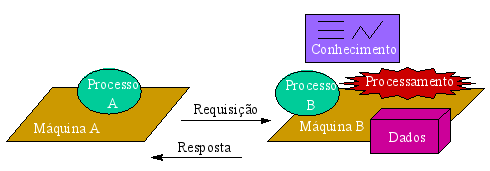
\includegraphics[width=0.9\textwidth]{./imagens/diagrama-cliente-servidor.png} % <- formatos PNG, JPG e PDF
	\caption[Paradigma Cliente-Servidor]{Paradigma Cliente-Servidor - Dados}
	\fonte{\cite{DBL98}}
	\label{fig:cliente-servidor}
\end{figure}

\begin{table}[htbp]
	\caption{Sistemas de Informação de Saúde do SUS}
	\label{tab:sus}
	\begin{tabular}{|p{4cm}|p{2.5cm}|p{4cm}|p{4cm}|}
		\hline
		SISTEMAS & EVENTO & INSTRUMENTO DE COLETA & UTILIZAÇÃO \\ \hline
		SIM - Sistema de Informações sobre Mortalidade & Óbito & Declaração de Óbito & Estudos de mortalidade, vigilância de óbitos (infantil, materno). \\ \hline
		SINASC - Sistema de Informações sobre Nascidos Vivos & Nascido Vivo & Declaração de Nascido Vivo & Monitoramento da saúde da criança, vigilância da criança de risco. \\ \hline
		SINAN - Sistema de Informações de Agravos Notificáveis & Agravos Sob Notificação & Fichas Individuais de Notificação e Investigação & Acompanhamento dos agravos sob notificação, surtos, epidemias. \\ \hline
		SIH - Sistema de Informações Hospitalares & Informação Hospitalar & Autorização de Internação Hospitalar & Morbidade hospitalar, gestão hospitalar, custeio da atenção hospitalar. \\ \hline
		SAI - Sistema de Informações Ambulatorial & Produção Ambulatorial & Boletim de Produção Ambulatorial & Acompanhamento da produção ambulatorial, gestão Ambulatorial custeio da atenção ambulatorial. \\ \hline
		SISVAN - Sistema de Vigilância Alimentar e Nutricional & Estado Nutricional & Cartão da Criança e Cartão da Gestante & Estado nutricional de crianças de zero a cinco anos e gestantes. \\ \hline
		API - Avaliação do Programa de Imunizações & Vacinas Aplicadas & Boletim Mensal de Doses Aplicadas & Contém informações referentes às doses de vacinas aplicadas. \\ \hline
	\end{tabular}
	\fonte{\cite{sus2001}}
\end{table}
%-------------------------------------------------------------------------------


A seguir ilustra-se a forma de incluir figuras, tabelas, equa\c{c}\~oes, siglas e s\'imbolos no documento, obtendo indexa\c{c}\~ao autom\'atica em suas respectivas listas. A numera\c{c}\~ao sequencial de figuras, tabelas e equa\c{c}\~oes ocorre de modo autom\'atico. Refer\^encias cruzadas s\~ao obtidas atrav\'es dos comandos {\ttfamily \textbackslash label\{\}} e {\ttfamily \textbackslash ref\{\}}. Por exemplo, n\~ao \'e necess\'ario saber que o n\'umero deste cap\'itulo \'e~\ref{chap:revbib} para colocar o seu n\'umero no texto. Isto facilita muito a inser\c{c}\~ao, remo\c{c}\~ao ou reloca\c{c}\~ao de elementos numerados no texto (fato corriqueiro na escrita e corre\c{c}\~ao de um documento acad\^emico) sem a necessidade de renumer\'a-los todos.

\section{Figuras}

Na figura~\ref{fig:dummy} \'e apresentado um exemplo de gr\'afico flutuante. Esta figura aparece automaticamente na lista de figuras. Para uso avan\c{c}ado de gr\'aficos no \LaTeX, recomenda-se a consulta de literatura especializada~\cite{Goossens2007}.


\begin{figure}[!htb]
	\centering
	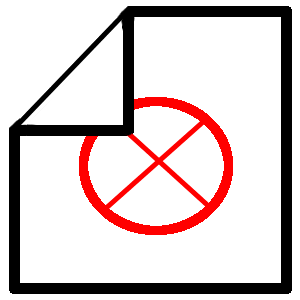
\includegraphics[width=0.2\textwidth]{./imagens/dummy.png} % <- formatos PNG, JPG e PDF
	\caption[Exemplo de uma figura]{Exemplo de uma figura onde aparece uma imagem sem nenhum significado especial.}
	\fonte{\cite{abnTeX2009}}
	\label{fig:dummy}
\end{figure}


\section{Tabelas}

% Trecho extraído do modelo http://www2.dainf.ct.utfpr.edu.br/ppgca/estrutura-academica/regulamentacao/avaliacao/copy_of_ModeloProjetoeSeminarios.doc/view
O título de uma tabela deve estar acima da mesma (ver tabela \ref{tab:patologias}).

\begin{table}[htbp]
	\centering
	\caption{Percentual das patologias identificadas nos prontuários analisados de 2003 a 2005}
	\label{tab:patologias}
	\begin{tabular}{|c|c|}
		\hline
		PATOLOGIAS IDENTIFICADAS & PERCENTUAL (\%) \\ \hline
		Lesão sobre o Nervo Femoral & 3,40\% \\ \hline
		Espondilolistese Lombar & 7,90\% \\ \hline
		Encurtamento Muscular Lombar & 9,60\% \\ \hline
		Alteração Muscular em MMII & 17,50\% \\ \hline
		Comprometimento Sacro-Ilíaca & 2,80\% \\ \hline
		Disfunção Neurológica Radicular Cervical & 9,00\% \\ \hline
		Síndrome do Desfiladeiro Torácico & 2,30\% \\ \hline
		Lombalgia & 27,70\% \\ \hline
		Cervicalgia & 19,80\% \\ \hline
	\end{tabular}
	\fonte{\cite{LAP05}}
\end{table}

%-------------------------------------------------------------------------------

Tamb\'em \'e apresentado o exemplo da tabela~\ref{tab:correlacao}, que aparece automaticamente na lista de tabelas. Informa\c{c}\~oes sobre a constru\c{c}\~ao de tabelas no \LaTeX\ podem ser encontradas na literatura especializada~\cite{Lamport1986,Buerger1989,Kopka2003,Mittelbach2004}.

\begin{table}[!htb]
	\centering
	\caption[Exemplo de uma tabela]{Exemplo de uma tabela mostrando a correla\c{c}\~ao entre x e y.}
	\label{tab:correlacao}
	\begin{tabular}{cc}
		\hline 
		x & y \\
		\hline
		1 & 2 \\
		3 & 4 \\
		5 & 6 \\
		7 & 8 \\
		\hline 
	\end{tabular}
	\fonte{Autoria pr\'opria.}
\end{table}

\section{Equa\c{c}\~oes}

A transformada de Laplace \'e dada na equa\c{c}\~ao~(\ref{eq:laplace}), enquanto a equa\c{c}\~ao~(\ref{eq:dft}) apresenta a formula\c{c}\~ao da transformada discreta de Fourier bidimensional\footnote{Deve-se reparar na formata\c{c}\~ao esteticamente perfeita destas equa\c{c}\~oes!}.

\begin{equation}
X(s) = \int\limits_{t = -\infty}^{\infty} x(t) \, \text{e}^{-st} \, dt
\label{eq:laplace}
\end{equation}

\begin{equation}
F(u, v) = \sum_{m = 0}^{M - 1} \sum_{n = 0}^{N - 1} f(m, n) \exp \left[ -j 2 \pi \left( \frac{u m}{M} + \frac{v n}{N} \right) \right]
\label{eq:dft}
\end{equation}

\section{Siglas e s\'imbolos}

O pacote \textsc{abn}\TeX\ permite ainda a defini\c{c}\~ao de siglas e s\'imbolos com indexa\c{c}\~ao autom\'atica atrav\'es dos comandos {\ttfamily \textbackslash sigla\{\}\{\}} e {\ttfamily \textbackslash simbolo\{\}\{\}}. Por exemplo, o significado das siglas\sigla{CPGEI}{Programa de P\'os-gradua\c{c}\~ao em Engenharia El\'etrica e Inform\'atica Industrial},\sigla{DAELN}{Departamento Acad\^emico de Eletr\^onica} e\sigla{UTFPR}{Universidade Tecnol\'ogica Federal do Paran\'a} aparecem automaticamente na lista de siglas, bem como o significado dos s\'imbolos\simbolo{$\lambda$}{comprimento de onda},\simbolo{$v$}{velocidade} e\simbolo{$f$}{frequ\^encia} aparecem automaticamente na lista de s\'imbolos. Mais detalhes sobre o uso destes e outros comandos do \textsc{abn}\TeX\ s\~ao encontrados na sua documenta\c{c}\~ao espec\'ifica~\cite{abnTeX2009}.

% Trecho extraído do modelo http://www2.dainf.ct.utfpr.edu.br/ppgca/estrutura-academica/regulamentacao/avaliacao/copy_of_ModeloProjetoeSeminarios.doc/view
Elemento opcional elaborado de acordo com a ordem apresentada no texto, seguido do significado correspondente. Caso não haja símbolos, não é necessário incluir a lista de símbolos.

Adaptação para usar comando \\simbolo{}
% Lista de símbolos matemáticos: http://web.ift.uib.no/Fysisk/Teori/KURS/WRK/TeX/symALL.html

\begin{itemize}
	\item \simbolo{$\bar{x}$}{Tempo médio de uma amostra}: Tempo médio de uma amostra.
	\item \simbolo{$\sigma$}{Desvio Padrão}: Desvio Padrão.
	\item \simbolo{$n$}{Número de valores da amostra}: Número de valores da amostra.
	\item \simbolo{$\Delta$}{Variação do intervalo de confiança de 95\% para a estimação da média da população}: Variação do intervalo de confiança de 95\% para a estimação da média da população.
\end{itemize}


%-------------------------------------------------------------------------------

\chapter{Metodologia}
\label{chap:metod}

% Trecho extraído do modelo http://www2.dainf.ct.utfpr.edu.br/ppgca/estrutura-academica/regulamentacao/avaliacao/copy_of_ModeloProjetoeSeminarios.doc/view
Outros títulos muitos comuns para esse capítulo são MÉTODOS ou MATERIAIS E MÉTODOS.
É uma descrição técnica de como será desenvolvido ou foi desenvolvido o trabalho. Devem estar detalhadas, de forma lógica, linear e cronológica, todas as etapas do projeto.
Uma metodologia bem estruturada reflete um bom planejamento do processo de investigação, diminuindo a possibilidade de surgirem falhas que impeçam a conclusão do projeto.
A metodologia contempla, entre outros: como será feito o levantamento bibliográfico, indicando as áreas a serem estudadas e critérios de inclusão e exclusão da literatura; o tipo do estudo; o local onde será desenvolvido; a população, a amostra selecionada e os critérios adotados; a coleta de dados (instrumentos e procedimentos de coleta); o desenvolvimento do aparato tecnológico em questão, como, por exemplo, software ou hardware; análise dos dados; aspectos éticos envolvidos na pesquisa. Os modelos de questionários, entrevistas e materiais complementares utilizados podem ser apresentados nos resultados ou em apêndices, quando de autoria do aluno, ou em anexos, quando de autoria de terceiros.
Eventualmente, durante a descrição, serão necessárias justificativas para a escolha de um ou outro método, e, mesmo que o projeto proponha uma metodologia inédita, as referências bibliográficas devem ser apresentadas.
A abordagem que será utilizada para a análise dos resultados também deve ser explicitada, indicando o teste estatístico ou processo analítico que permitirá a extração de conclusões.
É importante deixar bem claro o processo de avaliação e validação dos resultados a serem obtidos. Não basta apenas dizer que o será avaliado, sendo necessário descrever detalhadamente todo o processo de avaliação, bem como descrever o processo de validação.
A metodologia é que efetivamente demonstra o caminho selecionado e trilhado pelo pesquisador para materializar o trabalho e atingir os objetivos propostos, devendo, portanto, ser clara e detalhadamente descrita.
Devem ser descritas as alterações entre a metodologia apresentada no Projeto de Dissertação de Mestrado e nos Seminários de Acompanhamento I e II (caso hajam).
%-------------------------------------------------------------------------------
\chapter{Resultados}
\label{chap:result}

% Trecho extraído do modelo http://www2.dainf.ct.utfpr.edu.br/ppgca/estrutura-academica/regulamentacao/avaliacao/copy_of_ModeloProjetoeSeminarios.doc/view
Aqui serão apresentados os resultados obtidos (parciais ou finais). Contudo, não será discutido aqui se os resultados são adequados, inadequados, bons, ruins, entre outros. Ou seja, os resultados deverão ser desprovidos de interpretação. A avaliação e a validação planejadas na metodologia serão demonstradas aqui, passo a passo, até a indicação dos resultados. Na documento de dissertação final deverá haver resultados para cada objetivo apresentado anteriormente (para o geral e para os específicos).
Os resultados podem ser apresentados sob a forma de, entre outros: tabelas; figuras; fotografias ou outras representações gráficas que complementem o texto; questionários formulados; modelagem de software (análise orientada a objetos), circuitos de hardware.
Devem ser descritas as alterações entre os resultados apresentados no Projeto de Dissertação de Mestrado e nos Seminários de Acompanhamento I e II (caso haja).

%-------------------------------------------------------------------------------
\chapter{Discuss\~ao}
\label{chap:disc}

% Trecho extraído do modelo http://www2.dainf.ct.utfpr.edu.br/ppgca/estrutura-academica/regulamentacao/avaliacao/copy_of_ModeloProjetoeSeminarios.doc/view

As discussões poderão incluir, entre outros: análise dos resultados obtidos; discussões envolvendo as implicações dos resultados; discussões sobre os resultados que parecem contradizer as expectativas originais.

%-------------------------------------------------------------------------------
\chapter{Conclus\~ao}
\label{chap:concl}

Espera-se que o uso do estilo de formata\c{c}\~ao \LaTeX\ adequado \`as Normas para Elabora\c{c}\~ao de Trabalhos Acad\^emicos da UTFPR ({\ttfamily normas-utf-tex.cls}) facilite a escrita de documentos no \^ambito desta institui\c{c}\~ao e aumente a produtividade de seus autores. Para usu\'arios iniciantes em \LaTeX, al\'em da bibliografia especializada j\'a citada, existe ainda uma s\'erie de recursos~\cite{CTAN2009} e fontes de informa\c{c}\~ao~\cite{TeX-Br2009,Wikibooks2009} dispon\'iveis na Internet.

Recomenda-se o editor de textos Kile como ferramenta de composi\c{c}\~ao de documentos em \LaTeX\ para usu\'arios Linux. Para usu\'arios Windows recomenda-se o editor \TeX nicCenter~\cite{TeXnicCenter2009}. O \LaTeX\ normalmente j\'a faz parte da maioria das distribui\c{c}\~oes Linux, mas no sistema operacional Windows \'e necess\'ario instalar o software \textsc{MiK}\TeX~\cite{MiKTeX2009}.

Al\'em disso, recomenda-se o uso de um gerenciador de refer\^encias como o JabRef~\cite{JabRef2009} ou Mendeley~\cite{Mendeley2009} para a cataloga\c{c}\~ao bibliogr\'afica em um arquivo \textsc{Bib}\TeX, de forma a facilitar cita\c{c}\~oes atrav\'es do comando {\ttfamily \textbackslash cite\{\}} e outros comandos correlatos do pacote \textsc{abn}\TeX. A lista de refer\^encias deste documento foi gerada automaticamente pelo software \LaTeX\ + \textsc{Bib}\TeX\ a partir do arquivo {\ttfamily reflatex.bib}, que por sua vez foi composto com o gerenciador de refer\^encias JabRef.

O estilo de formata\c{c}\~ao \LaTeX\ da UTFPR e este exemplo de utiliza\c{c}\~ao foram elaborados por Diogo Rosa Kuiaski (diogo.kuiaski@gmail.com) e Hugo Vieira Neto (hvieir@utfpr.edu.br), com contribui\c{c}\~oes de C\'esar Vargas Benitez. Sugest\~oes de melhorias s\~ao bem-vindas.

% Trecho extraído do modelo http://www2.dainf.ct.utfpr.edu.br/ppgca/estrutura-academica/regulamentacao/avaliacao/copy_of_ModeloProjetoeSeminarios.doc/view
As conclusões do trabalho devem ser expostas de maneira clara, lógica e concisa, devendo fundamentar o que foi obtido na discussão. Deverá haver correspondência entre as conclusões e os objetivos específicos propostos no início do trabalho.
Deve haver um relacionamento com a Introdução, onde está a hipótese do trabalho, fechando desta forma o ciclo de desenvolvimento do trabalho. Mais especificamente, as conclusões devem responder aos objetivos específicos.

\section{Trabalhos Futuros}
Indicar aqui os vários trabalhos que podem ser incentivados e realizados a partir deste. Este tópico deve demonstrar que o trabalho desenvolvido não se encerra em si mesmo, mostrando o caminho a ser seguido pelos próximos trabalhos.
%-------------------------------------------------------------------------------
\chapter{Informa\c{c}\~oes Complementares}
\label{chap:infcompl}

% Trecho extraído do modelo http://www2.dainf.ct.utfpr.edu.br/ppgca/estrutura-academica/regulamentacao/avaliacao/copy_of_ModeloProjetoeSeminarios.doc/view
Neste capítulo constará uma série de informações que se destinam a subsidiar os membros das bancas do Projeto de Dissertação de Mestrado e dos Seminários de Acompanhamento I e II. 
Na versão final da dissertação este capítulo deverá desaparecer e, apresentando alguma informação pertinente e necessária ao conteúdo da dissertação, esta deverá ser transferida para o local apropriado na dissertação.

\section{Or\c{c}amento}
Aqui deve ser apresentada toda a relação de material permanente e de consumo que será utilizado no projeto, a sua quantidade, o seu custo (caso seja gratuito, indicar a gratuidade) e o financiador. Caso estes materiais, permanentes ou de consumo, e equipamentos não estejam disponíveis na Universidade Tecnológica Federal do Paraná (UTFPR), o pesquisador deve informar como irá obtê-los ou a entidade que os possui e que possa disponibilizá-los para a sua pesquisa. A aprovação do Projeto de Dissertação de Mestrado, ou dos Seminários de Acompanhamento I ou II, não garante nenhuma forma de financiamento adicional.
Materiais de consumo que fazem parte do arsenal trivial de um laboratório ou serviço devem ser também listados e orçados, independentemente da quantidade a ser utilizada.

\section{Dificuldades encontradas}
Aqui devem ser descritas as dificuldades encontradas na realização no trabalho, bem como os caminhos adotados para superá-las.

\section{Etapas e Cronograma}
Apresentação através de texto, tabela, planilha ou esquema, da distribuição das várias etapas do projeto ao longo do período previsto para sua execução. O cronograma deverá permitir uma visão ampla do projeto, de seus objetivos, e suas etapas, facilitando a identificação das atribuições de todos os participantes do projeto.

\subsection{Etapas}
Sugere-se que o cronograma seja organizado em etapas conforme o seguinte modelo:

\begin{table}[htbp]
	\centering
	\begin{tabular}{|c|p{8cm}|}
		\hline
		NOME DA ETAPA & DESCRIÇÃO DA ETAPA \\ \hline
		Etapa 1 & Descrição da etapa  \\ \hline
		Etapa 2 & Descrição da etapa  \\ \hline
		... & ... \\ \hline
		Etapa n & Descrição da etapa n \\ \hline
	\end{tabular}
	\caption{Etapas do Projeto}
	\label{quadro:etapas}
\end{table}

O número de etapas varia conforme o projeto. Caso haja variação entre as etapas apresentadas em documentos anteriores, as diferenças devem ser apresentas também.

\subsection{Cronograma mensal das etapas de desenvolvimento do trabalho}

Deverão ser apresentadas as tarefas programadas e as realizadas no momento da entrega do Pré-Projeto de Dissertação de Mestrado ou do Projeto de Dissertação de Mestrado. A seguir é apresentada uma sugestão de representação de cronograma. Caso seja necessário, o quadro deve ser dividido.


\begin{table}[htbp]
	\begin{tabular}{|p{3cm}|p{0.07cm}|p{0.07cm}|p{0.07cm}|p{0.07cm}|p{0.07cm}|p{0.07cm}|p{0.07cm}|p{0.07cm}|p{0.07cm}|p{0.07cm}|p{0.07cm}|p{0.07cm}|p{0.07cm}|p{0.07cm}|p{0.07cm}|p{0.07cm}|p{0.07cm}|p{0.07cm}|p{0.07cm}|p{0.07cm}|p{0.07cm}|p{0.07cm}|p{0.07cm}|p{0.07cm}|p{0.07cm}|}
		\hline
		\multicolumn{ 2}{|l|}{\textbf{Ano}} & \multicolumn{ 10}{c|}{\textbf{200...}} & \multicolumn{ 12}{c|}{\textbf{200...}} & \multicolumn{ 2}{c|}{\textbf{200...}} \\ \hline
		\multicolumn{ 2}{|l|}{\textbf{Etapas / Mês}} & \textbf{M} & \textbf{A} & \textbf{M} & \textbf{J} & \textbf{J} & \textbf{A} & \textbf{S} & \textbf{O} & \textbf{N} & \textbf{D} & \textbf{J} & \textbf{F} & \textbf{M} & \textbf{A} & \textbf{M} & \textbf{J} & \textbf{J} & \textbf{A} & \textbf{S} & \textbf{O} & \textbf{N} & \textbf{D} & \textbf{J} & \textbf{F} \\ \hline
		Nome da etapa 1 & P & \textbf{X} & \textbf{X} & \textbf{X} & \textbf{} & \textbf{} & \textbf{} & \textbf{} & \textbf{} & \textbf{} & \textbf{} & \textbf{} & \textbf{} & \textbf{} & \textbf{} & \textbf{} & \textbf{} & \textbf{} & \textbf{} & \textbf{} & \textbf{} & \textbf{} & \textbf{} & \textbf{} & \textbf{} \\ \hline
		\textbf{} & \textbf{R} & \textbf{X} & \textbf{X} & \textbf{} & \textbf{} & \textbf{} & \textbf{} & \textbf{} & \textbf{} & \textbf{} & \textbf{} & \textbf{} & \textbf{} & \textbf{} & \textbf{} & \textbf{} & \textbf{} & \textbf{} & \textbf{} & \textbf{} & \textbf{} & \textbf{} & \textbf{} & \textbf{} & \textbf{} \\ \hline
		Nome da etapa 2 & P & \textbf{} & \textbf{X} & \textbf{X} & \textbf{X} & \textbf{} & \textbf{} & \textbf{} & \textbf{} & \textbf{} & \textbf{} & \textbf{} & \textbf{} & \textbf{} & \textbf{} & \textbf{} & \textbf{} & \textbf{} & \textbf{} & \textbf{} & \textbf{} & \textbf{} & \textbf{} & \textbf{} & \textbf{} \\ \hline
		\textbf{} & \textbf{R} & \textbf{} & \textbf{X} & \textbf{X} & \textbf{X} & \textbf{} & \textbf{} & \textbf{} & \textbf{} & \textbf{} & \textbf{} & \textbf{} & \textbf{} & \textbf{} & \textbf{} & \textbf{} & \textbf{} & \textbf{} & \textbf{} & \textbf{} & \textbf{} & \textbf{} & \textbf{} & \textbf{} & \textbf{} \\ \hline
		... & P & \textbf{} & \textbf{} & \textbf{} & \textbf{} & \textbf{} & \textbf{} & \textbf{} & \textbf{X} & \textbf{X} & \textbf{X} & \textbf{} & \textbf{} & \textbf{} & \textbf{} & \textbf{} & \textbf{} & \textbf{} & \textbf{} & \textbf{} & \textbf{} & \textbf{} & \textbf{} & \textbf{} & \textbf{} \\ \hline
		\textbf{} & \textbf{R} & \textbf{} & \textbf{} & \textbf{} & \textbf{} & \textbf{} & \textbf{} & \textbf{} & \textbf{} & \textbf{X} & \textbf{X} & \textbf{} & \textbf{} & \textbf{} & \textbf{} & \textbf{} & \textbf{} & \textbf{} & \textbf{} & \textbf{} & \textbf{} & \textbf{} & \textbf{} & \textbf{} & \textbf{} \\ \hline
		Nome da etapa n & P & \textbf{} & \textbf{} & \textbf{} & \textbf{} & \textbf{} & \textbf{} & \textbf{} & \textbf{} & \textbf{} & \textbf{} & \textbf{} & \textbf{} & \textbf{} & \textbf{} & \textbf{} & \textbf{} & \textbf{} & \textbf{} & \textbf{} & \textbf{} & \textbf{} & \textbf{} & \textbf{X} & \textbf{X} \\ \hline
		\textbf{} & \textbf{R} & \textbf{} & \textbf{} & \textbf{} & \textbf{} & \textbf{} & \textbf{} & \textbf{} & \textbf{} & \textbf{} & \textbf{} & \textbf{} & \textbf{} & \textbf{} & \textbf{} & \textbf{} & \textbf{} & \textbf{} & \textbf{} & \textbf{} & \textbf{} & \textbf{} & \textbf{X} & \textbf{X} & \textbf{} \\ \hline
	\end{tabular}
	\caption{Cronograma. P: Programado; R: Realizado}
	\label{tab:cronograma}
\end{table}

%-------------------------------------------------------------------------------
\chapter{Refer\^encias}
\label{chap:ref}

% Trecho extraído do modelo http://www2.dainf.ct.utfpr.edu.br/ppgca/estrutura-academica/regulamentacao/avaliacao/copy_of_ModeloProjetoeSeminarios.doc/view

Todas as referências citadas no texto devem estar relacionadas em ordem alfabética, conforme os exemplos descritos a seguir, que seguem as normas da ABNT. Não devem ser apresentadas referências que não foram citadas no texto.
A referência é um conjunto padronizado de elementos descritivos, retirados de um documento, que permitem sua identificação individual (ASSOCIAÇÃO BRASILEIRA DE NORMAS TÉCNICAS, 2000). As referências devem estar alinhadas à margem esquerda do texto, utilizando espaço simples e separadas umas das outras por dois espaços simples (ASSOCIAÇÃO BRASILEIRA DE NORMAS TÉCNICAS, 2000).
A seguir estão representados alguns exemplos para referências bibliográficas. As normas da ABNT podem ser consultadas em site específico da Biblioteca da UTFPR: \\ \url{http://www.utfpr.edu.br/curitiba/biblioteca-e-producao-academica/ normas-para-elaboracao-de-trabalhos-academicos} . 

LIVROS

SOBRENOME(S) DO(S) AUTORES(ES), Prenome (S) (iniciais ou por extenso). Título da obra: subtítulo. Edição. Local de publicação (Cidade): Editora, data de publicação. Paginação.

Exemplos:

SILVEIRA, I.C. da. O pulmão na prática médica. Rio de Janeiro: Vozes, 1993. 159 p.


LANGE, Danny B.; OSHIMA, Mitsuru. Programming and Deploying Java Mobile Agents with Aglets. Estados Unidos da América: Addison-Wesley, 1998. 227 p.


CAPÍTULO DE LIVRO

SOBRENOME(S) DO(S) AUTOR(ES) da parte referenciada, Prenome (S) (iniciais ou por extenso). Título da parte referenciada. In: SOBRENOMES (S) DO(S) AUTOR(ES) (ou editor, etc), Prenome(s) (iniciais ou por extenso) da publicação. Título da publicação: subtítulo. Edição. Local de publicação (Cidade): Editora, data de publicação. Capítulo, páginas (inicial e final).


Exemplo:

ESPOSITO, G. Os segredos do abismo. In: GOMES, V. A vida abissal. Curitiba: Champanhat, 1932, p. 151-178.


ARTIGOS DE PERIÓDICOS

SOBRENOME(S) DO(S) AUTOR(ES), Prenome (S) (iniciais ou por extenso). Título do artigo: subtítulo. Título da publicação, Local de publicação (Cidade), volume, fascículo, página inicial e final do artigo, periódico e data de publicação.


Exemplos:

MOURA, A.S. de. Direito de habitação às classes de baixa renda. Ciência \& Trópico, Recife, v. 11, n. 1, p. 71-78, 1983.


FERREIRA, Christina Ramires; LOPES, Maria Denise. Complexo hiperplasia cística endometrial/piometra em cadelas – revisão. Clínica veterinária, São Paulo, v. 5, n. 27, p. 36-44, jul. 2000.


MONOGRAFIAS

SOBRENOME(S) DO(S) AUTOR(ES), Prenome (S) (iniciais ou por extenso). Título da obra: subtítulo. Edição. Local de publicação (Cidade): Editora, data de publicação. Paginação.


Exemplos:
GORDON, Richard. A assustadora história da medicina. 5. ed. Rio de Janeiro: Ediouro, 1996. 223 p.


MEGGINSON, Leon C.; MOSLEY, Donald C.; PIETR JR, Paul H. Administração: conceitos e aplicações. 4. ed. São Paulo: Harbra,1998. 614 p.


DISSERTAÇÕES E TESES

SOBRENOME(S) DO(S) AUTOR(ES), Prenome (S) (iniciais ou por extenso). Título da dissertação ou tese: subtítulo. Data (ano de depósito). Folhas. Grau de dissertação ou tese – Unidade onde foi defendida, Local, data (ano da defesa).


Exemplos:

FREITAS, S.R.C. de. Marés gravimétricas: implicações para a placa sul-americana. 1993. 264p. Dissertação (Mestrado em Geofísica) – Instituto Astronômico e Geofísico, Universidade de São Paulo, São Paulo, 1993.


PEIXOTO, Luciano Almeida. Sistema de Apoio à Decisão em Exames Ortopédicos da Coluna Vertebral para Auxílio nos Diagnósticos Fisioterapêuticos das Regiões Cervical e Lombar. 2005. 102p. Dissertação (Mestrado em Tecnologia em Saúde) - Programa de Pós-Graduação em Tecnologia em Saúde, Pontifícia Universidade Católica do Paraná, Curitiba, 2005.


FANTUCCI, I. Contribuição do alerta, da atenção, da intenção e da expectativa temporal para o desempenho de humanos em tarefas de tempo de reação. 2001. 130 p. Tese (Doutorado em Psicologia) – Instituto de Psicologia, Universidade de São Paulo, São Paulo, 2001.


PUBLICAÇÃO DE AUTORIA DESCONHECIDA

pRIMEIRA palavra do título em maiúscula: subtítulo. Edição. Local de publicação (Cidade): Editora, data de publicação. Paginação.


Exemplos:

DESARROLLO energético em América Latina y la economia mundial. Santiago: Ed. Universitária, 1980. 245 p.


Sistema de Informação em Saúde. <http:////www.saude.sc.gov.br// sala\_de\_leitura//artigos//Sistemas\_de\_Informacao//SistemasInformaçãoSaúde.doc>. Acesso em de março de 2001.


ARTIGOS DE JORNAIS

SOBRENOME(S) DO(S) AUTOR(ES), Prenome (S) (iniciais ou por extenso). Título da matéria: subtítulo. Título do Jornal, Local de publicação (Cidade), data de publicação. Seção, caderno ou parte do jornal, página inicial e final do artigo ou matéria.


Exemplos:

SUZUKI JR., M. A melhor de todas as copas. Folha de S. Paulo, 02 jul. 1998. Caderno 4, Copa 98, p. 1.


NAVES, P. Lagos andinos dão banho de beleza. Folha de São Paulo, São Paulo, 28 jun. 1999. Folha Turismo, Caderno 8, p. 13.


NORMAS TÉCNICAS

ORGÃO NORMALIZADOR. Título: subtítulo, número da Norma. Local de publicação (Cidade), data de publicação. Paginação.


Exemplo:

ASSOCIAÇÃO BRASILEIRA DE NORMAS TÉCNICAS. Informação e documentação – referências – elaboração: NBR 6023. Rio de Janeiro, 2000. 356 p.


ARTIGOS DE PERIÓDICOS DISPONÍVEIS EM MEIO ELETRÔNICO

SOBRENOME(S) DO(S) AUTOR(ES), Prenome (S) (iniciais ou por extenso). Título do artigo: subtítulo. Título da publicação. Disponível em: <endereço eletrônico> Acesso em: data (25 dez. 1999).


Exemplo:

JUNIOR, Lopes; LIMA, Aury Celso de. A prisão de Pinochet e a extraterritorialidade da lei penal. Boletim Paulista de Direito. Disponível em: <http://www.jus.com.br/links/revista.html>. Acesso em: 28 fev. 1999.


CONSTITUIÇÃO FEDEREAL

PAÍS. ESTADO ou MUNICÍPIO. Constituição (data de promulgação). Título. Local: Editor, Ano de publicação. Número de páginas ou volumes. Notas.


Exemplo:

BRASIL. Constituição (1988). Constituição da República Federativa do Brasil. Brasília, DF: Senado, 1988.


LEIS E DECRETOS 

PAÍS, ESTADO ou MUNICÍPIO. Lei ou Decreto, número, data (dia, mês e ano). Ementa. Dados da publicação que publicou a lei ou decreto.


Exemplos:

BRASIL. Lei n. 9610, de 19 de fevereiro de 1998. Dispõe sobre os direitos autorais.

BRASIL. Lei n. 6.895, de 17 de dezembro de 1980. Dá nova redação aos arts. 184 e 186 do Código Penal, aprovado pelo Decreto-lei nº 2.848, de 7 de dezembro de 1940. Diário Oficial da União de 18 de dezembro de 1980.
%-------------------------------------------------------------------------------

\bibliography{reflatex} % geracao automatica das referencias a partir do arquivo reflatex.bib
%---------- Apendices (opcionais) ----------
\apendice
\chapter{Nome do Ap\^endice}
\label{chap:apend}

Use o comando {\ttfamily \textbackslash apendice} e depois comandos {\ttfamily \textbackslash chapter\{\}}
para gerar t\'itulos de ap\^en-dices.

% Trecho extraído do modelo http://www2.dainf.ct.utfpr.edu.br/ppgca/estrutura-academica/regulamentacao/avaliacao/copy_of_ModeloProjetoeSeminarios.doc/view
Elemento opcional, que consiste em texto ou documento elaborado pelo autor, a fim de complementar sua argumentação, sem prejuízo da unidade nuclear do trabalho.
Os apêndices devem ser identificados por letras maiúsculas consecutivas, seguidas de travessão e respectivo título.
%-------------------------------------------------------------------------------

% ---------- Anexos (opcionais) ----------
\anexo
\chapter{Nome do Anexo}
\label{chap:anexo}

Use o comando {\ttfamily \textbackslash anexo} e depois comandos {\ttfamily \textbackslash chapter\{\}}
para gerar t\'itulos de anexos.

% Trecho extraído do modelo http://www2.dainf.ct.utfpr.edu.br/ppgca/estrutura-academica/regulamentacao/avaliacao/copy_of_ModeloProjetoeSeminarios.doc/view
Elemento opcional, que consiste em texto ou documento não elaborado pelo autor, que serve de fundamentação, comprovação e ilustração.
Os anexos devem ser identificados por letras maiúsculas consecutivas, seguidas de travessão e respectivo título.
%-------------------------------------------------------------------------------


% --------- Lista de siglas --------
\chapter{Lista de siglas}
\label{chap:siglas}

% Trecho extraído do modelo http://www2.dainf.ct.utfpr.edu.br/ppgca/estrutura-academica/regulamentacao/avaliacao/copy_of_ModeloProjetoeSeminarios.doc/view
Elemento opcional, constituída de uma relação alfabética das abreviaturas e siglas utilizadas no texto, seguido das palavras ou expressões correspondentes grafadas por extenso. Quando necessário, recomenda-se a elaboração de lista própria para cada tipo. Caso não haja abreviaturas, não é necessário incluir a lista de abreviaturas. 

(Adaptado para usar o comando \\sigla)

\begin{itemize}
	\item \sigla{Bps}{bits por segundo}: bits por segundo
	\item \sigla{CGI}{Common Gateway Interface - Interface de Porta Comum}: Common Gateway Interface - Interface de Porta Comum
	\item \sigla{CNS}{Cartão Nacional de Saúde}: Cartão Nacional de Saúde
\end{itemize}

%-------------------------------------------------------------------------------

\textbf{* Observa\c{c}\~oes:} a lista de siglas nao realiza a ordenacao das siglas em ordem alfabetica
 Em breve isso sera implementado, enquanto isso: \\
\textbf{Sugest\~ao:} crie outro arquivo .tex para siglas e utilize o comando \textbackslash sigla\{sigla\}\{descri\c{c}\~ao\}.
Para incluir este arquivo no final do arquivo, utilize o comando \textbackslash input\{arquivo.tex\}.
Assim, Todas as siglas serao geradas na ultima pagina. Entao, devera excluir a ultima pagina da versao final do arquivo
 PDF do seu documento.


%-------- Citacoes ---------
% - Utilize o comando \citeonline{...} para citacoes com o seguinte formato: Autor et al. (2011).
% Este tipo de formato eh utilizado no comeco do paragrafo. P.ex.: \citeonline{autor2011}

% - Utilize o comando \cite{...} para citacoeses no meio ou final do paragrafo. P.ex.: \cite{autor2011}



%-------- Titulos com nomes cientificos (titulo, capitulos e secoes) ----------
% Regra para escrita de nomes cientificos:
% Os nomes devem ser escritos em italico, 
%a primeira letra do primeiro nome deve ser em maiusculo e o restante em minusculo (inclusive a primeira letra do segundo nome).
% VEJA os exemplos abaixo.
% 
% 1) voce nao quer que a secao fique com uppercase (caixa alta) automaticamente:
%\section[nouppercase]{\MakeUppercase{Estudo dos efeitos da radiacao ultravioleta C e TFD em celulas de} {\textit{Saccharomyces boulardii}}
%
% 2) por padrao os cases (maiusculas/minuscula) sao ajustados automaticamente, voce nao precisa usar makeuppercase e afins.
% \section{Introducao} % a introducao sera posta no texto como INTRODUCAO, automaticamente, como a norma indica.


\end{document}